\section{Overview Of Power Electronic}
\subsection{Introduction to Forward Converter} 
The Forward Converter is a type of isolated DC-DC converter widely used in medium-power applications (typically up to 200W). It provides electrical isolation between the input and output using a transformer, making it suitable for applications requiring safety, noise immunity, and flexibility. The forward converter is an evolution of the buck converter , with the addition of a transformer for isolation and energy transfer.
\subsubsection*{Key Features of the Forward Converter}
\begin{itemize}
    \item \textbf{Isolation:} The transformer provides galvanic isolation between the input and output, ensuring safety and preventing ground loops.
    
    \item \textbf{Step-Down Operation:} The forward converter steps down the input voltage to a lower output voltage, similar to a buck converter.
    
    \item \textbf{Continuous Conduction Mode (CCM):} Typically operates in Continuous Conduction Mode (CCM), where the inductor current never drops to zero during a switching cycle. This ensures high efficiency and low ripple.
    
    \item \textbf{Reset Mechanism:} A reset winding or active clamp circuit is used to reset the transformer core after each switching cycle, preventing core saturation.
    
    \item \textbf{Efficiency:} Achieves high efficiency due to minimal energy storage in the transformer.
    
    \item \textbf{Applications:} Suitable for medium-power applications (up to $\sim$200W), such as telecom power supplies, industrial equipment, and renewable energy systems.
\end{itemize}
\subsection{Purpose of the Report}
% \noindent % To make sure the text starts immediately after the multicolumn environment ends
\noindent The purpose of this report is to provide a comprehensive analysis of Forward converters, focusing on their working principle, key design considerations, and practical applications. By exploring these aspects, the report aims to highlight the technical nuances that make Forward converters indispensable in modern electronics while addressing challenges such as leakage inductance, switching losses, and electromagnetic interference (EMI).
\begin{figure}[h!]
    \centering
    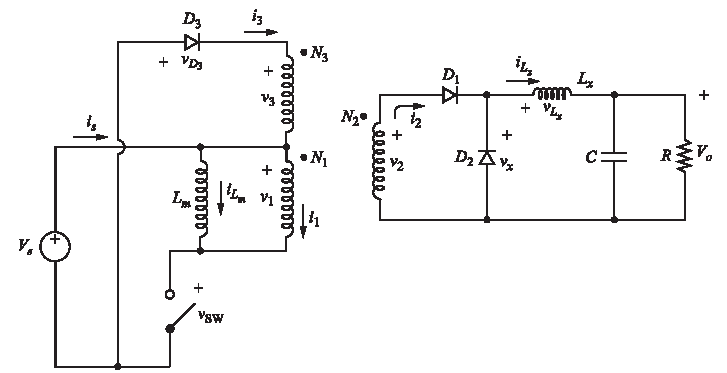
\includegraphics[width=0.7\linewidth]{Pictures/Images/1.pdf}
    \caption{\textcolor{blue}{\textit{\footnotesize Forward dc-dc converter}}}
\end{figure}
